\section{Design}

\subsection{Approach}

This chapter describes the high level design of Atmosphere platform, while the implementation details are described in later chapters. 

So far we’ve discussed the current state of SaaS client applications and their problems. We’ve come to the conclusion that the biggest issue with all client applications is that they block user interfaces with network requests. 

\subsubsection{Asynchronous interfaces}

This section defines the term asynchronous user interface.

In computer science, an asynchronous operation is such one, that doesn’t block the caller while being processed, but instead calls specified callback, or a delegate method, when completed.

Asynchronous interface is what we get by applying the same concept to users and interfaces. Users don’t want to be “blocked” (that means stare at the ‘loading’ title next to the spinning wheel) while their actions are being processed.

Asynchronous interface gives immediate response, and when processing is finished, it might present further results if needed.

The idea of asynchronous interface is well described in the article „Asynchronous Uis – the future of web user interfaces“ \citep{maccaw_async}

\subsubsection{Local Storage}

\begin{figure}[ht!]
\centering
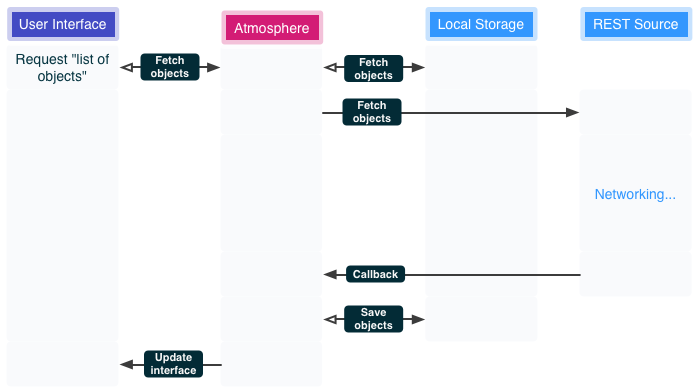
\includegraphics[width=400pt]{LocalStorage1.png}
\caption{Fetching objects using Atmosphere \label{fig:1}}
\end{figure}

Storing the data locally will help achieving an asynchronous interface. 

When user tries to access a set of objects, the application will first retrieve them from local storage, and then make a network request to retrieve the newest data. As soon as the data is retrieved from the server, Atmosphere will look at their unique identifiers and try to find an existing copy in the local storage. If the object is found, its attributes are updated and it’s saved back to the local storage. If it’s not, a new object is created locally.

The interface always displays local data. Using model-view bindings the interface is automatically updated whenever a change in local objects is made.

\begin{figure}[ht!]
\centering
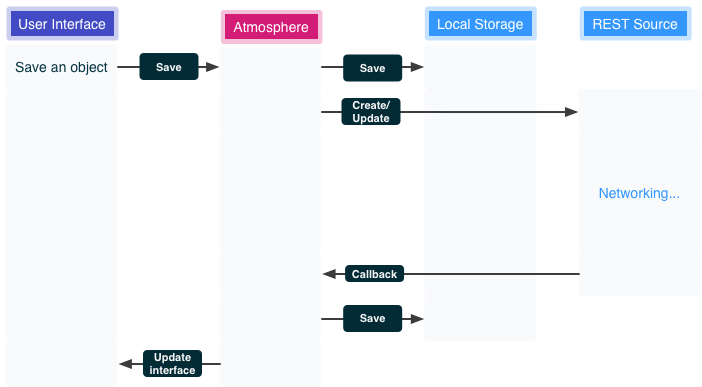
\includegraphics[width=400pt]{LocalStorage2.png}
\caption{Creating objects using Atmosphere \label{fig:2}}
\end{figure}

It works similarly the other way. When user creates a new object, or updates an existing object, the changes are immediately written to the local storage. At the same moment the object is marked as “changed locally”, and is scheduled for synchronization. The synchronization module picks it up, and sends it to the server.

Another important part of this process is deciding whether to send a “create” request or “update” request. For each object, Atmosphere keeps track of Boolean information “is local only”, which is set to true the first time object is created. At that point the object is assigned a temporary ID. When the object is successfully synchronized, it’s ID is updated to permanent ID assigned by the server and the value of “is local only” is set to false.

\subsubsection{Recovering from failure}

Network connection might be very unreliable in some cases. This problem is partly solved by keeping track of objects, which are local only. If the request is made, and it never comes back, the object is never unmarked as “local only” and the next synchronization cycle another create request is sent. 

A case that is not solved yet is the one when the network request is made, processed by the server, but the response never makes it back to the client. In such case the object is created remotely, but the client application isn’t informed about this: thus it tries to create the object again, which results in two objects of the same attributes.

Assigning permanent ID on the client side could solve this problem. Such solution would expect server to take ID as an argument to the create request. If such solution was in place, the previous case could be described as follows: A new object is created on the client side, it is assigned a temporary ID. Then it is sent to the server and server creates object with that ID. The response never comes back to the client, so client makes another create request, with the same ID. Server declines to create another object with the same ID, so it returns a confirmation message for existing object. This time client receives the confirmation message, so the object is marked as not local only. 

This solution is not implemented by Atmosphere because it would be implemented on the server side. Fortunately, it can be implemented very easily by adding very little code on the server side, and even less code on the server side. 

\subsubsection{Exceptions}

Always storing data locally whenever a new object is created might be harmful in certain cases.

For example a web commerce site might provide actions for adding products to the cart, and it might provide an action for submitting the order.

The programmer would probably decide to let Atmosphere manage creation of cart item object, but for order submission, they would probably want to make sure the order was submitted before updating user interface, possibly risking the user would close the window thinking they’re order was submitted while it was not.

For this purpose, Atmosphere implementations provide a way to create or update an object using a synchronous (in terms of user interface blocking) request. 

\subsubsection{Other solutions}

There are simpler ways of achieving asynchronous interface.

One of them would be to create transient objects that would represent remote objects and still hide networking from the user. Such solution would be less complex because there would have to be no synchronization.

 One drawback would be that opening application for the first time would be slow as user would have to wait for network request to complete. 

Another reason to use local storage and synchronization is that the application can be used offline.

\subsubsection{Notifications}

Atmosphere supports a notification system used for realtime updating of objects. This component is used by the server application using simple HTTP API. There are two types of notifications.

The first one is „object update“ type. The application server can send this  message to Atmosphere’s notification server to send live object update to connected clients. Such message should contain object’s attributes and list of users to send the notification to. Sending the „object update“ message will cause connected clients to update their local object with the new attributes sent by the server. Using bindings or some other technique, the user interface is updated and user sees the new attributes in real time.

The second type is „notification“ type. This message is also sent by the server, but instead of object attributes it contains a custom object to be passed to the connected clients. It also contains list of clients to send this message to. 

A „notification“ message will simply forward custom object to specified users. The client application is responsible for parsing and processing such message, Atmosphere will only provide a way for application to subscribe for these the notification messages. 

\subsection{Components}

\subsubsection{Client}

Client is the computer where Atmosphere-based application is running. It can be a web, desktop or a mobile application.

\begin{figure}[ht!]
\centering
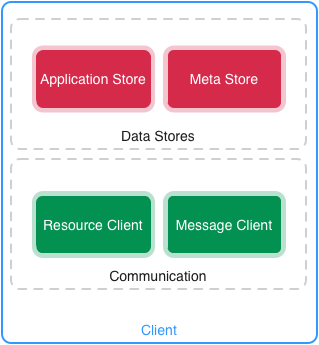
\includegraphics[width=200pt]{MainComponents.png}
\caption{Main components of the client \label{fig:3}}
\end{figure}

The implementions differ across platforms, but from a high level view there are two main component groups: One responsible for storing data locally and one responsible for communication with the HTTP server.

The Application Data Store is a component that is responsible for managing application objects. It is used for tasks like looking up an application object, or updating an application object. This component always depends on native way of storing data. In case of desktop applications, it depends on Core Data framework, etc. 

The Meta Store is a component that is responsible for storing meta objects, objects that encapsulate information that are needed by Atmosphere and that can be ignored by application itself.

List of meta data:

1. "is object changed" is a Boolean value that indicates whether the object was changed locally since the last synchronization. 

2. "is object local only" is a Boolean value that indicates, whether the object was retrieved from the server, or if it exists only in the local store. 

Components in the communication group are responsible for networking. Resource Client is component responsible for communication with the REST source while Message Client is responsible for communication with the Atmosphere notification server. 

\subsubsection{REST Source}

REST Source is an existing HTTP server. It is not important what language or technology is used to build this server, the only requirement for the server is to implement the basic CRUD methods: create, read, update and delete.

\begin{figure}[ht!]
\centering

\includegraphics[width=250pt]{RestSource.png}
\caption{Communication between the client and the REST source \label{fig:4}}
\end{figure}

The source can be also provided by a third party. For example, in application TaskDo (see section Case Study), the source is RESTful API of Google Tasks. 

Once the server is available and its methods are known, the client must be configured to use the correct methods to create, read, update and delete objects.

The communication between client and the REST source is then performed using HTTP methods.

\subsubsection{Notification server}

\begin{figure}[ht!]
\centering
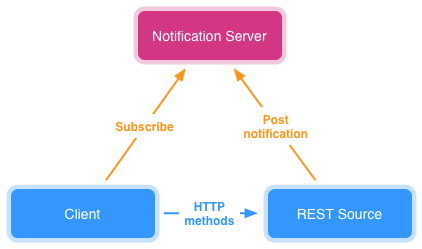
\includegraphics[width=250pt]{NotificationServer.png}
\caption{Use of the notification server by the client and the REST Source \label{fig:5}}
\end{figure}

Notification server is a component that stands between client application and REST source. Client subscribes to notifications on the notification server and the REST source posts notifications to the notification server. 